\documentclass[11pt]{article}

\usepackage{url}
\usepackage{hyperref}
\usepackage{graphicx}
\usepackage{verbatim}
\usepackage{color}
\setlength{\parskip}{0.5cm plus4mm minus3mm}
\usepackage{upquote}
\usepackage{float}

\textwidth=6.4in
\textheight=8.5in
\hoffset=-0.7in
\voffset=-0.7in

\setlength{\parindent}{0cm} 

\newcommand{\Yfun}{Y}
%\newcommand{\TAG}{test}
\newcommand{\TAG}{\begin{color}{blue}This tutorial is currently under construction. Please check back later for more by keeping your software updated.\end{color}}

\newcommand{\HERE}{\begin{color}{blue}Currently working on this part.\end{color}}

\hyphenation{Text-Wrangler}

\title{Chapter 2: Introduction to Slepian Functions}
\author{The Slepian Working Group}

\begin{document}
\maketitle

After having worked through Chapter 1: Introduction to Spherical
Harmonics, we will now have a look at what spherical Slepian functions
are. The goal of this chapter is not to give a solid foundation of the
mathematical intricacies. This can be obtained from the many research
articles in the literature. Rather, we will look at some basic ideas
and plot the first few Slepian functions.


\section{Basic ideas}
When plotting spherical harmonics in chapter 1, it became clear that
all of these spherical harmonics are functions that cover the entire
sphere. This is of course an advantage if we try to describe functions
(or maps), that cover the entire planet, such as gravity fields,
magnetic fields, etc. We saw in chapter 1 that we can generate pretty
much any spatial pattern we like by simply summing up different
spherical harmonics each multiplied by a different factor called
``coefficient''.

But what can we do if we only have information within a specific
region? Sometimes it's fine to just describe that information as
point values. But in some cases, as for example when we measure
gravity or magnetic data at satellite altitude, and we want to
calculate, what the corresponding magnetic or gravity field looks like
on the planet's surface (assuming there are no gravity or magnetic
sources between the planet and the satellite, or that they are
negligible), we need to describe these fields in spherical harmonics.

This is where the Slepian functions come in. Slepian functions are
linear combinations of spherical harmonics which means that they are
constructed by multiplying each spherical harmonic function with a
factor (called Slepian coefficient) and then adding them all up. The name
Slepian function stems from the first author of a research article,
that described the original idea for 1-dimensional functions.

There are different types of Slepian functions that are constructed in
different ways but the basic idea is always to solve an optimization
problem, in which we try to balance the number of spherical-harmonic
functions we use (the maximum spherical-harmonic degree) in the
construction of the Slepian functions, and how much they are
concentrated within the region that we are interested in.

\section{Classical Scalar Slepian Functions}
%A brief mathematical overview will be as follows; for a more in depth treatment, please see Section 2.3 of Simons and Plattner (2014): \\
%\url{https://pdfs.semanticscholar.org/886c/70532a885ca66c1b70e55eb65a3f6500be67.pdf}.
%
Let's first look at the classical scalar Slepian functions, which are spectrally limited and spatially optimized. These functions are suitable to use when you are limited to information within a specific region as mentioned above, but only when that information is constrained to the surface of the sphere as point values; vector Slepian functions will be addressed in a later section. The functions will be bandlimited by the maximum spherical harmonic degree \textit{L} for region of concentration \textit{R}. We will choose the continent \textbf{Africa} as \textit{R} for the following example in which we will calculate and plot spherical harmonic coefficients. 

\subsection{Example One - Using glmalpha() and plotting coefficients}

The function \verb+glmalpha+ is used to calculate unit-normalized spherical harmonic coefficients given the following required inputs:

\verb+TH+ - a desired region, in our case: \verb+'africa'+. This may also be any other spherical cap or ordered list defining a closed curve

\verb+L+ - the bandwidth, or maximum spherical harmonic degree

Thus the outputs of \verb+glmalpha+ we will need for this example are a unitary matrix of localization coefficients \verb+G+ and the eigenvalues \verb+V+. There are several other inputs and outputs that may and should be used; see \verb+help glmalpha+ for more details. 

We will specify one other input to indicate the ordering of the spherical harmonic coefficients. In our codes  we use two different methods of ordering: ADDMOUT and ADDMON. 

Remember that spherical harmonics have a degree $l$ and an order $m$. degrees are all integers greater than zero and orders for each degree vary between $-l$ and $l$.

We could order these spherical harmonics as


\begin{tabular}{c|cccccccccc}
l&0&1&1&1&2&2&2&2&2&etc.\\
\hline
m&0&-1&0&1&-2&-1&0&1&2&\text{etc.}
\end{tabular}

This is called the ADDMOUT ordering and is the ordering in which the columns of the Slepian matrices in \verb+glmalpha+, \verb+gradvecglmalpha+, and all these other similar functions are returned.

The other ordering that we are using is:

\begin{tabular}{c|cccccccccc}
l&0&1&1&1&2&2&2&2&2&\text{etc.}\\
\hline
m&0&0&-1&1&0&-1&1&-2&2&\text{etc.}
\end{tabular}

This one we call ADDMON and it is the ordering in which the coefficients from functions like \verb+LocalInnerField+ (which will be discussed in a later chapter) are returned. Every function that returns coefficients or matrices of coefficients should state in their help menu in which format the coefficients are.

Returning to our example we now know that \verb+glmalpha+ uses the ADDMOUT ordering and thus requires us to use \verb+0+ as the fourth input according to the help section. We will choose a value of \verb+L=20+. Now we can run:

\verb+[G,V] = glmalpha('africa',20,[],0)+

and observe the output \verb+G+ which should be a $(L+1)^2\times(L+1)^2$ orthonormal matrix of coefficients and \verb+V+ a single vector of eigenvalues.  

Once the coefficients have been calculated we desire a neutral type of sorting in the format called LMCOSI to prepare for plotting.

In the lmcosi format, we explicitly write out the degrees, orders, and coefficients which in the following I will call $c_{l\,m}$

\begin{tabular}{c c c c}
l&m&co&si\\
\hline
0&0&$c_{0\,0}$&0\\
1&0&$c_{1\,0}$&0\\
1&1&$c_{1\,-1}$&$c_{1\,1}$\\
2&0&$c_{2\,0}$&0\\
2&1&$c_{2\,-1}$&$c_{2\,1}$\\
2&2&$c_{2\,-2}$&$c_{2\,2}$\\
\vdots&\vdots&\vdots&\vdots
\end{tabular}

As you can see this last ordering is an entire matrix instead of just a vector. This is a disadvantage to run calculations but it is less ambiguous than just a vector of coefficients.


Luckily we have programs that take care of these issues. These programs have the creative names
\verb+coef2lmcosi+ and \verb+lmcosi2coef+. You can probably guess from the name what each does.

For our Africa example we will need to feed our coefficients into \verb+coef2lmcosi+ and again tell it whether they are in the ADDMOUT or ADDMON format. This is indicated by using the value 1 for the second input (see \verb+help coef2lmcosi+). The output is saved as \textit{lmcs} but you can name it whatever you would like. Run:

\verb+lmcs=coef2lmcosi(G(:,1),1)+

The first column of G is used for now because these are the spherical harmonic coefficients corresponding to the ``best" Slepian functions, or most spatially concentrated within our chosen region of Africa. \verb+G(:,2)+ would be the second best, \verb+G(:,3)+ would be the third best, and so on.

We now have one more step before we are ready to plot and that is to evaluate the coefficients using the function \verb+plm2xyz+. The required inputs are our \textit{lmcosi} format matrix and a chosen resolution. You can choose \textit{res}=1, or 0.5, or even 0.1 for a very high resolution image, but keep in mind this will also use much calculation time and memory.  We will give the output the arbitrary name `data' and choose  a resolution of 0.5. Run:

\verb+data=plm2xyz(lmcs,0.5)+

And finally to plot we will use \verb+plotplm+:

\verb+plotplm(data,[],[],4,0.5)+

for which our input choices follow the second input scheme of \verb+help plotplm+.

Run \verb+kelicol(1)+ for a more clear color scheme where white sections are of value 0, and you should see a map of Earth projected into a 2D plane with latitude as the y-axis and longitude on the x-axis. It is recommended to change the maximum and minimum of the color scheme which you can do by running:

\verb+caxis([-1,1]*max(abs(caxis)));+

As expected, the fluctuations are concentrated on the center of Africa and negligible elsewhere. Your plot should match that of Figure 1. \\

\begin{figure}[H]
  \centering
  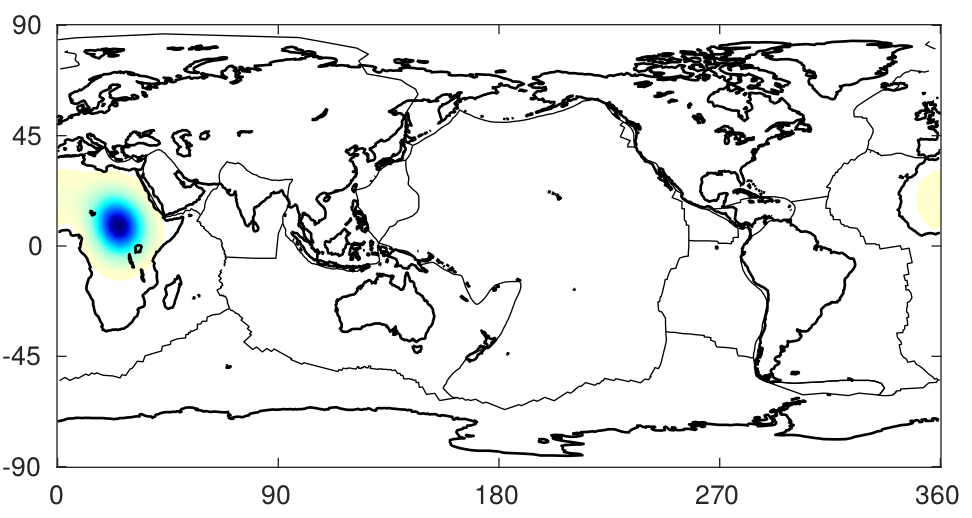
\includegraphics[width=0.5\textwidth]{figures/demoClassScaleAfrica.png}
  \caption{\begin{small}
  Result of example using glmalpha() with L=20 to calculate coefficients, plm2xyz() to evaluate them, and plotplm() to plot. The y-axis is latitude and x-axis is longitude. Only the first ``best" concentrated eigensolutions are plotted. The color scheme is kelicol(1) and max/min values are changed to fit the max/min of data plotted.
  \end{small}}
\label{plotplm}
\end{figure}

\textbf{Exercise:} Pick a different a region, or subtract a region from Africa to use as the domain and plot again. What do you see?
% clarify that plotplm can take either lmcosi or r lon lat data?
% add another example of regions subtracted
% add an exercise

\subsection{Example Two - Looking at Eigenvalues}

We will now take a look at our vector of eigenvalues, \verb+V+. You can plot the eigenvalues versus their corresponding rank $\alpha$ values by running the following:

\verb+plot(1:J,V)+

Where \verb|J=(L+1)^2|.

Using the \verb|V| from Example One we produce Figure 2 from which we can see that our eigenvalues drop off rapidly in value and become zero near $\alpha=50$. 

\begin{figure}[H]
  \centering
  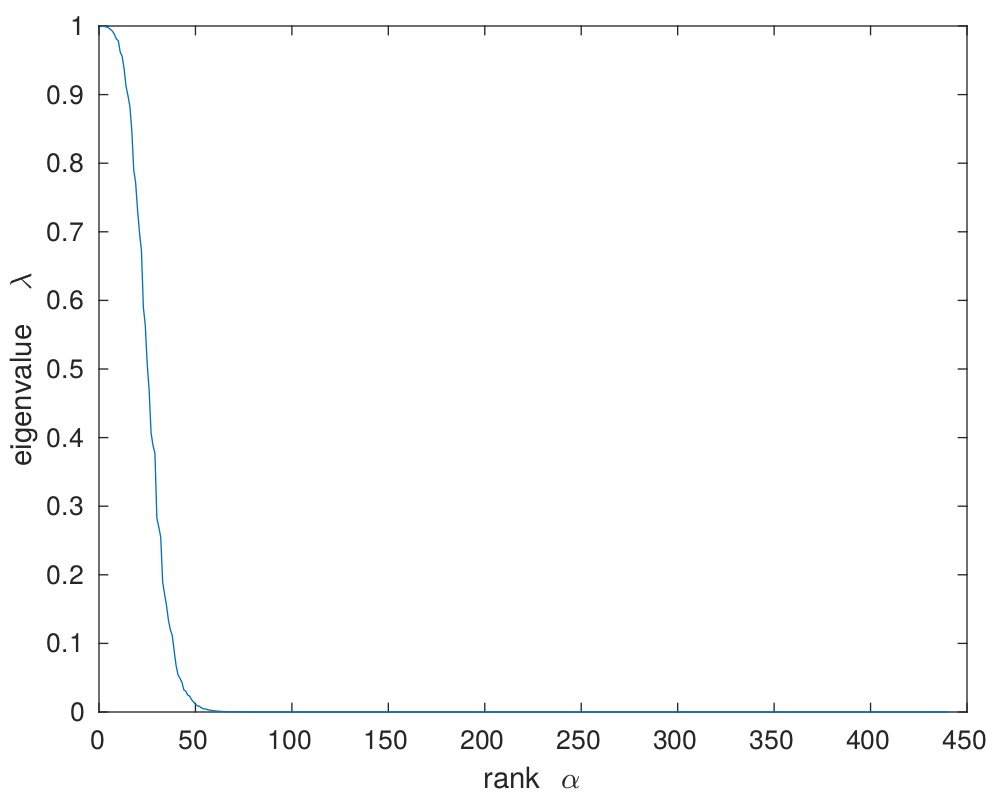
\includegraphics[width=0.5\textwidth]{figures/lambdaalphaplot.png}
  \caption{\begin{small}
  Eigenvalues plotted on the y-axis versus their corresponding rank on the x-axis. We can see that most of the energy is occuring in functions corresponding to $\alpha<50$. 
  \end{small}}
\label{vjdemoplot}
\end{figure}

Plotting this curve may be useful in selecting which eigensolutions will best represent the region of interest, as you will soon see.

Let's first plot the coefficients as we did in Example One, however this time we will plot all columns of \verb+G+. We can use a \verb+for+ loop to format each column of \verb+G+ in \textit{lmcosi}, evaluate the coefficients, and place each \textit{lmcosi} matrix as an element in the cell array \verb+g+:


\verb|for j=1:J| \\
\verb|    g{j} = plm2xyz(coef2lmcosi(G(:,j),1),.5)| \\
\verb|end| \\

We can then add the different elements of \verb+g+ into one matrix \verb|f|:

\verb|f = zeros*size(g{1}))| \\
\verb|for j=1:J| \\
\verb|    f = f + g{j}| \\
\verb|end| \\

and then plot with:

\verb|plotplm(f,[],[],4,.5)|

Your figure should match that of Figure 3. We can now see that using all of the eigensolutions may not be the best idea to represent our region of Africa.

\begin{figure}[H]
  \centering
  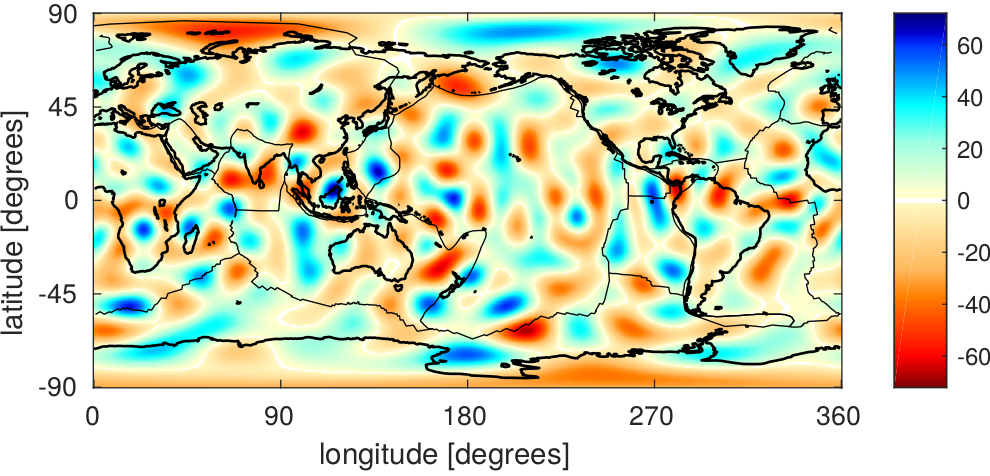
\includegraphics[width=0.5\textwidth]{figures/fplot.png}
  \caption{\begin{small}
  Using all eigensolutions to represent region Africa. L=20. 
  \end{small}}
\label{fplot}
\end{figure}

If we refer back to Figure 2 we can see that our eigenvalues drop off to zero around $\alpha=50$. Let's now reset \verb|J=50| and see what our plot looks like. You should be able to produce Figure 4, in which we see that our information has been concentrated within our region of choice, Africa.

\begin{figure}[H]
  \centering
  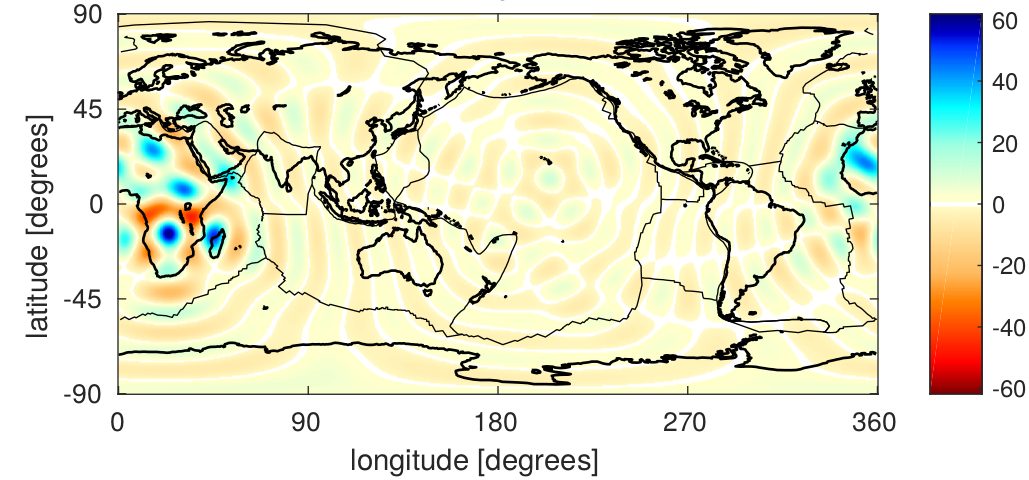
\includegraphics[width=0.5\textwidth]{figures/fJplot.png}
  \caption{\begin{small}
  Using all eigensolutions up to rank 50 to represent Africa.
  \end{small}}
\label{fJplot}
\end{figure}


\textbf{Exercise:} Create a vector of random numbers the same length as the matrix \verb|f| we plotted in Figure 4 and multiply it with \verb|g{j}| inside the \verb|for| loop. How does this change the plot when using the same eigensolutions? You should produce something similar to Figure 5.

\begin{figure}[H]
  \centering
  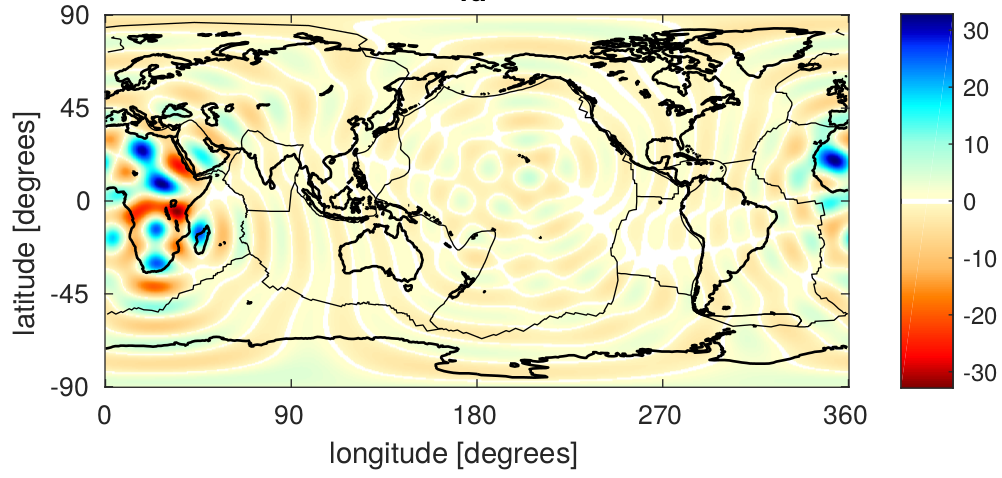
\includegraphics[width=0.5\textwidth]{figures/fuplot.png}
  \caption{\begin{small}
  Using eigensolutions up to rank 50 multiplied by a vector of random coefficients. 
  \end{small}}
\label{fuplot}
\end{figure}

****dont multiply g{j} times 1... multiply by random vector C ? ****** 
 

\TAG
\end{document}
